% !TeX root = surprises.tex

\selectlanguage{hebrew}
\chapter{איך לשמור על מוזיאון}
\label{c.museum}

ב-%
$1973$
\L{Victor Klee}
שאל כמה שומרים נחוצים כדי לראות את כל הקירות של מוזיאון על מנת לוודא שלא גונבים את הציורים. אם הקירות של המוזיאון מהווים מצולע משוכלל או אפילו מצולע קמור, אפשר להסתפק בשומר אחד:
\begin{center}
\selectlanguage{english}
\begin{tikzpicture}[scale=.8]
\coordinate (O) at (0,0);
\fill (O) circle (2pt);
\foreach \x/\name/\n/\po in {0/a/A/right,.6/b/B/above,1.6/c/C/left,2.4/d/D/below left,3.9/e/E/below right} {
  \coordinate (\name) at ($(O)+(\x*72+18:3cm)$);
%  \fill (\name) circle (1.5pt);
%  \node[\po] at (\name) {$\n$};
\draw[dashed] (O) -- (\name);
}
\draw (a) -- (b) -- (c) -- (d) --(e) -- cycle;
\end{tikzpicture}
\end{center}

מה עם מוזיאון עם קירות בצורה של מסור:

\begin{center}
\selectlanguage{english}
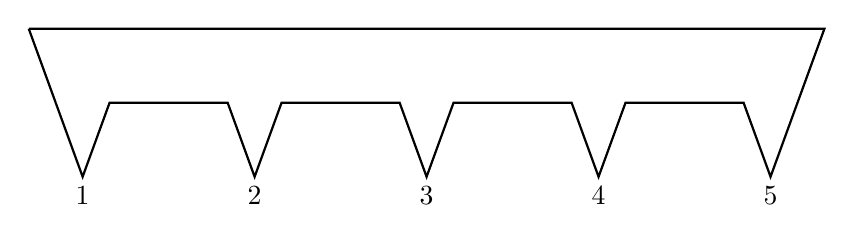
\begin{tikzpicture}[scale=1]
\coordinate (O) at (0,0);
\draw [thick] (O) -- (++110:1cm) coordinate (P);
\draw[thick] (O) --
  ++(-70:1cm) coordinate(A) node[below] {$1$} -- 
  ++(+70:1cm) -- ++(0:1.5cm) --
  ++(-70:1cm) coordinate(B) node[below] {$2$} -- 
  ++(+70:1cm) -- ++(0:1.5cm) --
  ++(-70:1cm) coordinate(C) node[below] {$3$}-- 
  ++(+70:1cm) -- ++(0:1.5cm) --
  ++(-70:1cm) coordinate(D) node[below] {$4$} -- 
  ++(+70:1cm) -- ++(0:1.5cm) --
  ++(-70:1cm) coordinate(E) node[below] {$5$} --
  ++(+70:2cm) -- (P);

\end{tikzpicture}
\end{center}

וודא על ידי ספירה שיש 
$15$
קירות.

כל "שן" של המסור מגדירה משולש )מסומן באפור(. שומרת הניצבת במקום כלשהו בתוך אחד המשולשים יכולה לראות את כל הקירות של אותו משולש:

\begin{center}
\selectlanguage{english}
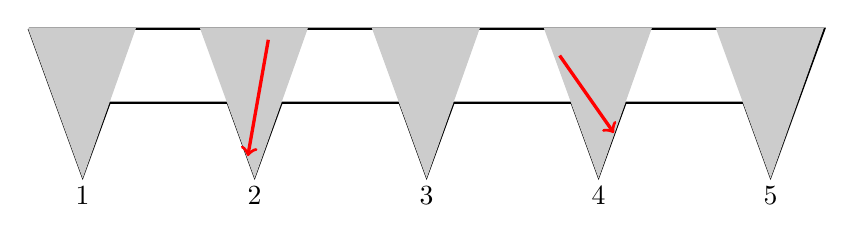
\begin{tikzpicture}[scale=1]
\coordinate (O) at (0,0);
\draw [thick] (O) -- (++110:1cm) coordinate (P);
\draw[thick] (O) --
  ++(-70:1cm) coordinate(A) node[below] {$1$} -- 
  ++(+70:1cm) -- ++(0:1.5cm) --
  ++(-70:1cm) coordinate(B) node[below] {$2$} -- 
  ++(+70:1cm) -- ++(0:1.5cm) --
  ++(-70:1cm) coordinate(C) node[below] {$3$}-- 
  ++(+70:1cm) -- ++(0:1.5cm) --
  ++(-70:1cm) coordinate(D) node[below] {$4$} -- 
  ++(+70:1cm) -- ++(0:1.5cm) --
  ++(-70:1cm) coordinate(E) node[below] {$5$} --
  ++(+70:2cm) -- (P);

\draw[fill,black!20!white] (A) -- ++(110:2cm) -- ++(0:1.35cm)-- cycle;
\draw[fill,black!20!white] (B) -- ++(110:2cm) -- ++(0:1.35cm)-- cycle;
\draw[fill,black!20!white] (C) -- ++(110:2cm) -- ++(0:1.35cm)-- cycle;
\draw[fill,black!20!white] (D) -- ++(110:2cm) -- ++(0:1.35cm)-- cycle;
\draw[fill,black!20!white] (E) -- ++(110:2cm) -- ++(0:1.35cm)-- cycle;

\draw[->,red,very thick] (2.7,.8) -- +(-100:1.5cm);
\draw[->,red,very thick] (6.4,.6) -- +(-55:1.2cm);
%\draw[->,very thick,green] (9,.9) -- (C);
%\draw[->,very thick,blue] ($(O)+(.5,.5)$) -- ++(7.5,.42);
%\draw[->,very thick,blue] ($(O)+(.5,.5)$) -- ++(3,-.5);
\end{tikzpicture}
\end{center}

אם השומרת ניצבת בקירבת הקיר העליון היא יכולה לראות את כל הקירות האופקיים )חצים כחולים(. ברור שחמש
שומרות מספיקות כדי לשמור על כל הקירות. אם המשולשים לא חופפים, שומרת במשולש אחד לא יכולה לראות את כל הקירות של משולש אחר )חץ ירוק(, לכן חייבים להעסיק חמש שומרות נחוצות.

\begin{center}
\selectlanguage{english}
\begin{tikzpicture}[scale=1]
\coordinate (O) at (0,0);
\draw [thick] (O) -- (++110:1cm) coordinate (P);
\draw[thick] (O) --
  ++(-70:1cm) coordinate(A) node[below] {$1$} -- 
  ++(+70:1cm) -- ++(0:1.5cm) --
  ++(-70:1cm) coordinate(B) node[below] {$2$} -- 
  ++(+70:1cm) -- ++(0:1.5cm) --
  ++(-70:1cm) coordinate(C) node[below] {$3$}-- 
  ++(+70:1cm) -- ++(0:1.5cm) --
  ++(-70:1cm) coordinate(D) node[below] {$4$} -- 
  ++(+70:1cm) -- ++(0:1.5cm) --
  ++(-70:1cm) coordinate(E) node[below] {$5$} --
  ++(+70:2cm) -- (P);

\draw[fill,black!20!white] (A) -- ++(110:2cm) -- ++(0:1.35cm)-- cycle;
\draw[fill,black!20!white] (B) -- ++(110:2cm) -- ++(0:1.35cm)-- cycle;
\draw[fill,black!20!white] (C) -- ++(110:2cm) -- ++(0:1.35cm)-- cycle;
\draw[fill,black!20!white] (D) -- ++(110:2cm) -- ++(0:1.35cm)-- cycle;
\draw[fill,black!20!white] (E) -- ++(110:2cm) -- ++(0:1.35cm)-- cycle;

%\draw[->,red,very thick] (2.7,1) -- (B);
\draw[->,very thick,green,dashed] (9,.8) -- +(-165:4.6cm);
\draw[->,very thick,blue] ($(O)+(.5,.5)$) -- ++(7.4,.4);
\draw[->,very thick,blue] ($(O)+(.5,.5)$) -- ++(2.9,-.45);
\draw (6,0) circle(4pt);
\draw (4.95,-.28) circle(4pt);
\end{tikzpicture}
\end{center}
\begin{theorem}\label{thm.guarded} \mbox{}\\
$\disfrac{n}{3}$
שומרות מספיקות ונחוצות כדי לשמור על כל מוזיאון עם
$n$
קירות.%
\footnote{אם 
$n$
לא מתחלק ב-%
$3$
מספר השומרות הנחוצות הוא 
$\left\lfloor \disfrac{n}{3}\right\rfloor$.
למשל,
$4$
שומרות מספיקות כדי לשמור על מוזיאונים עם
$12, 13, 14$
קירות כי
$\left\lfloor \disfrac{14}{3}\right\rfloor =\left\lfloor \disfrac{13}{3}\right\rfloor=\left\lfloor \disfrac{12}{3}\right\rfloor=4$.
לשם הפשטות נתעלם מסיבוך זה.}
\end{theorem}
ניתן להכליל את הדוגמה כדי להראות ש-%
$\disfrac{n}{3}$
שומרות נחוצות. שאר הפרק מוקדש להוכחה ש-%
$\disfrac{n}{3}$
מספיקות עבור כל מוזיאון.

\textbf{הגדרה:}
קודקוד במצולע הוא 
\textbf{קמור}
אם הזווית הפנימית פחות מ-%
$180^\circ$.
קודקוד במצולע הוא
\textbf{קעור}
אם הזווית הפנימית גדולה מ-%
$180^\circ$.

במצולע באיור להלן, קודקוד 
$1$
קמור וקודקוד
$2$
קעור.
\begin{center}
\selectlanguage{english}
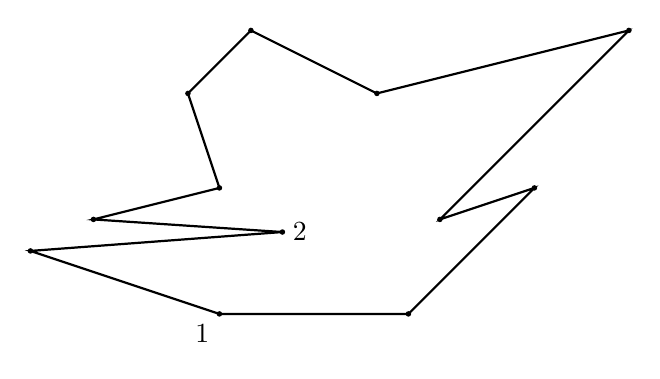
\begin{tikzpicture}[scale=.8]
\draw[thick]
  (0,0) coordinate (A) node[below left] {$1$} -- 
  ++(3,0) coordinate (B) --
  ++(2,2) coordinate (C) --
  ++(-1.5,-.5) coordinate (D) --
  ++(3,3) coordinate (E) -- 
  ++(-4,-1) coordinate (F) --
  ++(-2,1) coordinate (G) --
  ++(-1,-1) coordinate (H) --
  ++(.5,-1.5) coordinate (I) --
  ++(-2,-.5) coordinate (J) --
  ++(3,-.2) coordinate (K) node[right] {$2$} -- 
  ++(-4,-.3) coordinate (L) --
  cycle;
  
\foreach \point in {A,B,C,D,E,F,G,H,I,J,K,L}
  \fill (\point) circle(1.25pt);
\end{tikzpicture}
\end{center}
\textbf{הגדרה:}
ניתן
\textbf{לתלת}
\L{(triangulate)}
מצולע אם ניתן לצייר 
\textbf{אלכסונים},
קטעי קו שאינם נחתכים המחברים קודקודים והנמצאים בתוך המצולע לכל אורכם, כך שהשטח הפנימי של המצולע מכוסה על ידי משולשים זרים אחד מהשני.



\begin{theorem}\label{thm.tri}\mbox{}\\
ניתן לתלת כל מצולע.
\end{theorem}
אנו דוחים את ההוכחה של משפט~%
\ref{thm.tri}
לשלב מאוחר יותר.
\textbf{הגדרה:}
ניתן
\textbf{לצבוע מצולע בשלושה צבעים}
אם קיים מיפוי
\[
c: V \mapsto \{\textrm{\R{אדום, כחול, ירוק}}\}
\]
כך ששני הקודקודים של צלע מקבלים צבעים שונים.
\begin{theorem}\mbox{}\\
ניתן לצבוע מצולע מתולת בשלושה צבעים.
\label{thm.colored}
\end{theorem}
\textbf{הוכחה:}
באינדוקציה על מספר הקודקודים. ברור שניתן לצבוע משולש בשלושה צבעים. ניתן מצולע עם 
$n>3$
קודקודים. חייבים לצייר לפחות אלכסון אחד כדי לתלת את המצולע. בחר אלכסון שרירותי
$\overline{AB}$:

\begin{center}
\selectlanguage{english}
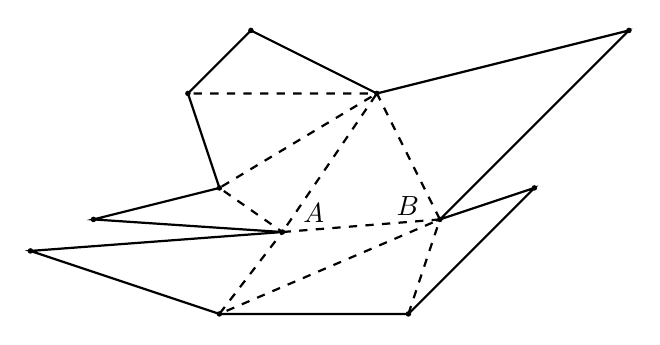
\begin{tikzpicture}[scale=.8]
\draw[thick]
  (0,0) coordinate (A) -- 
  ++(3,0) coordinate (B) --
  ++(2,2) coordinate (C) --
  ++(-1.5,-.5) coordinate (D) --
  ++(3,3) coordinate (E) -- 
  ++(-4,-1) coordinate (F) --
  ++(-2,1) coordinate (G) --
  ++(-1,-1) coordinate (H) --
  ++(.5,-1.5) coordinate (I) --
  ++(-2,-.5) coordinate (J) --
  ++(3,-.2) coordinate (K) -- 
  ++(-4,-.3) coordinate (L) --
  cycle;
  
\foreach \point in {A,B,C,D,E,F,G,H,I,J,K,L}
  \fill (\point) circle(1.25pt);

\node[above right,xshift=4pt] at (K) {$A$};
\node[above left,xshift=-4pt,yshift=-2pt] at (D) {$B$};

\draw[thick,dashed]
  (B) -- (D) -- (K) -- (F) -- (I) -- (K) -- (A) -- (D) -- (F) -- (H);
\end{tikzpicture}
\end{center}
וחלק את המצולע לאורך אלכסון זה לשני מצולעים קטנים יותר:
\begin{center}
\selectlanguage{english}
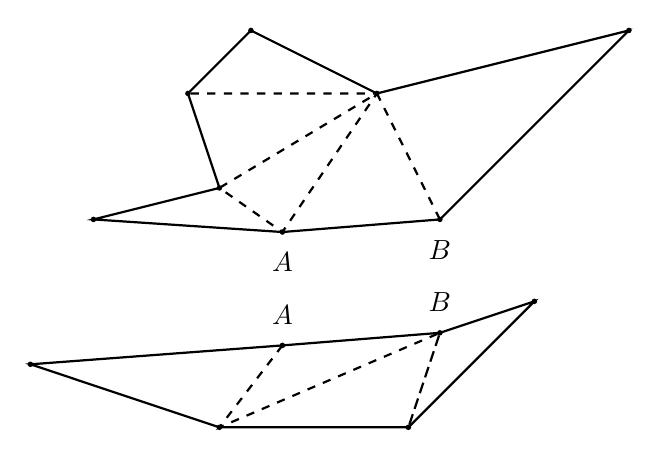
\begin{tikzpicture}[scale=.8]
\path
  (0,0) coordinate (A1) -- 
  ++(3,0) coordinate (B1) --
  ++(2,2) coordinate (C1) --
  ++(-1.5,-.5) coordinate (D1);
\draw[thick]
  (D1) --
  ++(3,3) coordinate (E1) -- 
  ++(-4,-1) coordinate (F1) --
  ++(-2,1) coordinate (G1) --
  ++(-1,-1) coordinate (H1) --
  ++(.5,-1.5) coordinate (I1) --
  ++(-2,-.5) coordinate (J1) --
  ++(3,-.2) coordinate (K1);
\path
  (K1) -- 
  ++(-4,-.3) coordinate (L1) --
  (A1);
  
\foreach \point in {D1,E1,F1,G1,H1,I1,J1,K1}
  \fill (\point) circle(1.25pt);

\node[below,yshift=-4pt] at (K1) {$A$};
\node[below,yshift=-4pt] at (D1) {$B$};

\draw[thick,dashed]
  (D1) -- (F1) -- (I1) -- (K1) -- (F1) -- (H1);
\draw[thick] (D1) -- (K1);

\begin{scope}[yshift=-1.8cm]

\draw[thick]
  (0,0) coordinate (A2) -- 
  ++(3,0) coordinate (B2) --
  ++(2,2) coordinate (C2) --
  ++(-1.5,-.5) coordinate (D2);
\path
  (D2) --
  ++(3,3) coordinate (E2) --
  ++(-4,-1) coordinate (F2) --
  ++(-2,1) coordinate (G2) --
  ++(-1,-1) coordinate (H2) --
  ++(.5,-1.5) coordinate (I2) --
  ++(-2,-.5) coordinate (J2) --
  ++(3,-.2) coordinate (K2);
\draw[thick]
  (K2) --
  ++(-4,-.3) coordinate (L2) --
  (A2);
  
\foreach \point in {A2,B2,C2,D2,K2,L2}
  \fill (\point) circle(1.25pt);
  
\node[above,yshift=4pt] at (K2) {$A$};
\node[above,yshift=4pt] at (D2) {$B$};

\draw[thick,dashed]
  (K2) -- (A2) -- (D2) -- (B2) -- (D2);
\draw[thick] (D2) -- (K2);

\end{scope}
\end{tikzpicture}
\end{center}
לפי הנחת האינדוקציה, ניתן לצבוע כל אחד מהמצולעים הללו בשלושה צבעים:
\begin{center}
\selectlanguage{english}
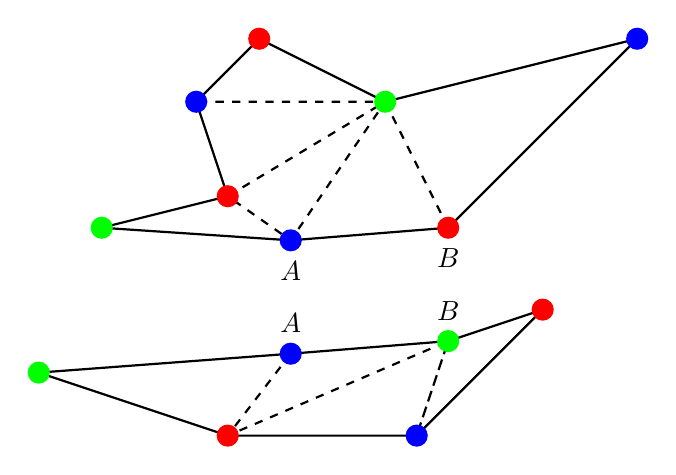
\begin{tikzpicture}[scale=.8]
\path
  (0,0) coordinate (A1) -- 
  ++(3,0) coordinate (B1) --
  ++(2,2) coordinate (C1) --
  ++(-1.5,-.5) coordinate (D1);
\draw[thick]
  (D1) --
  ++(3,3) coordinate (E1) -- 
  ++(-4,-1) coordinate (F1) --
  ++(-2,1) coordinate (G1) --
  ++(-1,-1) coordinate (H1) --
  ++(.5,-1.5) coordinate (I1) --
  ++(-2,-.5) coordinate (J1) --
  ++(3,-.2) coordinate (K1);
\path
  (K1) -- 
  ++(-4,-.3) coordinate (L1) --
  (A1);
  
\draw[thick,dashed]
  (D1) -- (F1) -- (I1) -- (K1) -- (F1) -- (H1);
\draw[thick] (D1) -- (K1);

\node[below,yshift=-4pt] at (K1) {$A$};
\node[below,yshift=-4pt] at (D1) {$B$};

\foreach \point/\color in {D1/red,E1/blue,F1/green,G1/red,H1/blue,I1/red,J1/green,K1/blue}
  \fill[color=\color] (\point) circle(5pt);


\begin{scope}[yshift=-1.8cm]

\draw[thick]
  (0,0) coordinate (A2) -- 
  ++(3,0) coordinate (B2) --
  ++(2,2) coordinate (C2) --
  ++(-1.5,-.5) coordinate (D2);
\path
  (D2) --
  ++(3,3) coordinate (E2) --
  ++(-4,-1) coordinate (F2) --
  ++(-2,1) coordinate (G2) --
  ++(-1,-1) coordinate (H2) --
  ++(.5,-1.5) coordinate (I2) --
  ++(-2,-.5) coordinate (J2) --
  ++(3,-.2) coordinate (K2);
\draw[thick]
  (K2) --
  ++(-4,-.3) coordinate (L2) --
  (A2);
  
\draw[thick,dashed]
  (K2) -- (A2) -- (D2) -- (B2) -- (D2);
\draw[thick] (D2) -- (K2);
\node[above,yshift=4pt] at (K2) {$A$};
\node[above,yshift=4pt] at (D2) {$B$};

\foreach \point/\color in {A2/red,B2/blue,C2/red,D2/green,K2/blue,L2/green}
  \fill[color=\color] (\point) circle(5pt);


\end{scope}
\end{tikzpicture}
\end{center}
השיוך של צבעים לקודקודים הוא שרירותי, כך שאם הקודקודים 
$A,B$
מקבלים צבעים שונים בשני המצולעים, ניתן לשנות את הצבעים באחד מהם כך שהצבעים של 
$A,B$
זהים בשני המצולעים. נחליף את הצבעים
\textbf{אדום}
ו-%
\textbf{ירוק}
במצולע התחתון:
\begin{center}
\selectlanguage{english}
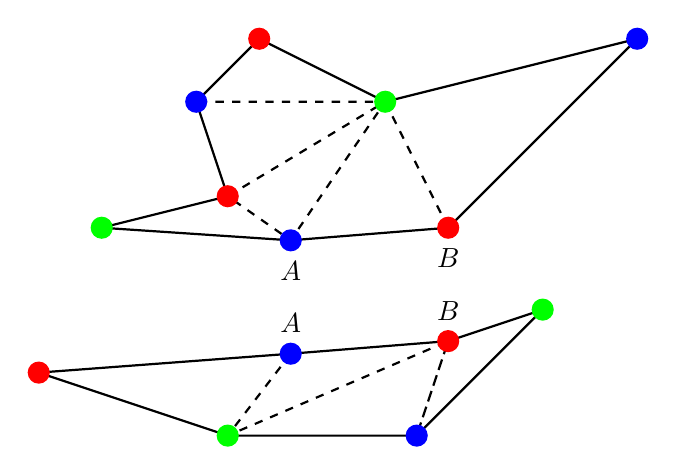
\begin{tikzpicture}[scale=.8]
\path
  (0,0) coordinate (A1) -- 
  ++(3,0) coordinate (B1) --
  ++(2,2) coordinate (C1) --
  ++(-1.5,-.5) coordinate (D1);
\draw[thick]
  (D1) --
  ++(3,3) coordinate (E1) -- 
  ++(-4,-1) coordinate (F1) --
  ++(-2,1) coordinate (G1) --
  ++(-1,-1) coordinate (H1) --
  ++(.5,-1.5) coordinate (I1) --
  ++(-2,-.5) coordinate (J1) --
  ++(3,-.2) coordinate (K1);
\path
  (K1) -- 
  ++(-4,-.3) coordinate (L1) --
  (A1);
  
\node[below,yshift=-4pt] at (K1) {$A$};
\node[below,yshift=-4pt] at (D1) {$B$};

\draw[thick,dashed]
  (D1) -- (F1) -- (I1) -- (K1) -- (F1) -- (H1);
\draw[thick] (D1) -- (K1);
\foreach \point/\color in {D1/red,E1/blue,F1/green,G1/red,H1/blue,I1/red,J1/green,K1/blue}
  \fill[color=\color] (\point) circle(5pt);

\begin{scope}[yshift=-1.8cm]

\draw[thick]
  (0,0) coordinate (A2) -- 
  ++(3,0) coordinate (B2) --
  ++(2,2) coordinate (C2) --
  ++(-1.5,-.5) coordinate (D2);
\path
  (D2) --
  ++(3,3) coordinate (E2) --
  ++(-4,-1) coordinate (F2) --
  ++(-2,1) coordinate (G2) --
  ++(-1,-1) coordinate (H2) --
  ++(.5,-1.5) coordinate (I2) --
  ++(-2,-.5) coordinate (J2) --
  ++(3,-.2) coordinate (K2);
\draw[thick]
  (K2) --
  ++(-4,-.3) coordinate (L2) --
  (A2);
  

\draw[thick,dashed]
  (K2) -- (A2) -- (D2) -- (B2) -- (D2);
\draw[thick] (D2) -- (K2);
\node[above,yshift=4pt] at (K2) {$A$};
\node[above,yshift=4pt] at (D2) {$B$};


\foreach \point/\color in {A2/green,B2/blue,C2/green,D2/red,K2/blue,L2/red}
  \fill[color=\color] (\point) circle(5pt);

\end{scope}
\end{tikzpicture}
\end{center}
כעת ניתן להדביק את שני המצולעים ביחד כדי לשחזר את המצולע המקורי עם
$n$
קודקודים. המצולע יהיה צבוע בשלושה צבעים.
\qed
\begin{center}
\selectlanguage{english}
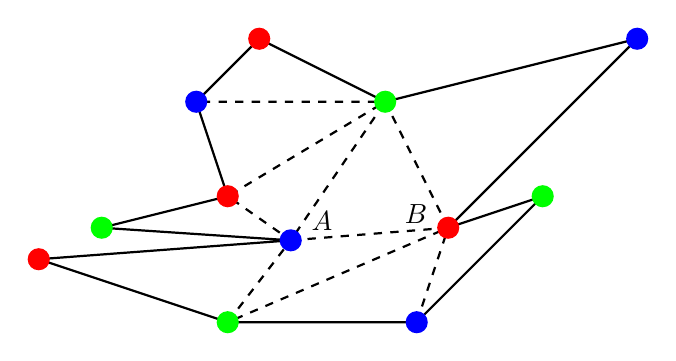
\begin{tikzpicture}[scale=.8]
\draw[thick]
  (0,0) coordinate (A) -- 
  ++(3,0) coordinate (B) --
  ++(2,2) coordinate (C) --
  ++(-1.5,-.5) coordinate (D) --
  ++(3,3) coordinate (E) -- 
  ++(-4,-1) coordinate (F) --
  ++(-2,1) coordinate (G) --
  ++(-1,-1) coordinate (H) --
  ++(.5,-1.5) coordinate (I) --
  ++(-2,-.5) coordinate (J) --
  ++(3,-.2) coordinate (K) -- 
  ++(-4,-.3) coordinate (L) --
  cycle;
  

\node[above right,xshift=4pt] at (K) {$A$};
\node[above left,xshift=-4pt,yshift=-2pt] at (D) {$B$};

\draw[thick,dashed]
  (B) -- (D) -- (K) -- (F) -- (I) -- (K) -- (A) -- (D) -- (F) -- (H);

\foreach \point/\color in {D/red,E/blue,F/green,G/red,H/blue,I/red,J/green,K/blue,A/green,B/blue,C/green,L/red}
  \fill[color=\color] (\point) circle(5pt);
\end{tikzpicture}
\end{center}


\textbf{הוכחה של משפט
\ref{thm.guarded}:}
לפי משפט
\ref{thm.tri}
ניתן לתלת את המצולע ולפי משפט
\ref{thm.colored}
ניתן לצבוע את המצולע בשלושה צבעים. שלושת הקודקודים של כל משולש יהיו צבועים בצבעים שונים, כך שכל צבע מופיע באחד הקודקודים של כל משולש. אם צובעים 
$n$
קודקודים בשלושה צבעים, צבע אחד לפחות )נניח אדום( מופיע לכל היותר
$\disfrac{n}{3}$
פעמים, ובכל משולש חייב להיות קודקוד צבוע אדום.

אם נציב שומרת בקודקוד אדום, היא יכולה לראות את הקירות של אותו משולש. כל המשולשים של תילות המצולע כוללים את כל הצלעות של המצולע, ולכן
$\disfrac{n}{3}$
שומרות מספיקות כדי לראות את כל הקירות של המוזיאון.
\qed

כעת נוכיח את משפט
\ref{thm.tri}
שניתן לתלת כל מצולע.

\begin{theorem}\mbox{}\\
סכום הזוויות הפנימיות של מצולע עם
$n$
צלעות הוא
$180^\circ(n-2)$.
\end{theorem}

\newpage

\textbf{הוכחה:}
תחילה נוכיח עבור מצולעים קמורים. נסמן את 
\textbf{הזוויות החיצוניות}
ב-%
$\theta_i$:
\begin{center}
\selectlanguage{english}
\begin{tikzpicture}[scale=.6]
\coordinate (O) at (0,0);
%\fill (O) circle (2pt);
\foreach \x/\name/\n/\po in {0/a/A/right,.6/b/B/above,1.6/c/C/left,2.4/d/D/below left,3.9/e/E/below right} {
  \coordinate (\name) at ($(O)+(\x*72+18:3cm)$);
%  \fill (\name) circle (1.5pt);
%  \node[\po] at (\name) {$\n$};
%\draw[dashed] (O) -- (\name);
}
\draw[thick] (a) -- (b) -- (c) -- (d) --(e) -- cycle;

\draw[thick,dashed] (a) 
  node[above,xshift=-2pt,yshift=8pt] {$\theta_1$} -- 
  ($(a)!2!(b)$);
\draw[thick,dashed] (b)
  node[above left,xshift=-8pt,yshift=0pt] {$\theta_2$} -- 
  ($(b)!1.7!(c)$);
\draw[thick,dashed] (c) 
  node[below left,xshift=-4pt,yshift=-2pt] {$\theta_3$} -- 
  ($(c)!1.7!(d)$);
\draw[thick,dashed] (d)
  node[below right,xshift=0pt,yshift=-4pt] {$\theta_4$} -- 
  ($(d)!1.5!(e)$);
\draw[thick,dashed] (e)
  node[right,xshift=4pt,yshift=4pt] {$\theta_5$} -- 
  ($(e)!1.7!(a)$);

\end{tikzpicture}
\end{center}
אם נסכם את הזוויות החיצוניות נקבל 
$\displaystyle\sum_{i=1}^n \theta_i = 360^\circ$.
ניתן לראות את הסיכום באיור על ידי "סיבוב" הקווים המקווקווים מאחד לשני לפי הסדר 
$\theta_1,\ldots,\theta_5$.
עבור כל זוית חיצונית
$\theta_i$
נסמן את הזוית הפנימית של אותו קודקוד ב-%
$\phi_i$.
נחשב:
\erh{2pt}\begin{equationarray*}{rcl}
\displaystyle\sum_1^n \theta_i &=&\displaystyle\sum_1^n (180^\circ-\phi_i)= 360^\circ\\
%n\cdot 180^\circ-\displaystyle\sum_1^n \phi_i &=& 360^\circ\\
\displaystyle\sum_1^n \phi_i &=& n\cdot 180^\circ-360^\circ =180^\circ(n-2)\,.
\end{equationarray*}
נבדוק מה קורה אם נוסיף קודקוד קעור:
\begin{center}
\selectlanguage{english}
\begin{tikzpicture}
\draw[thick] (0,0) -- (3,0) coordinate (A) node[above left,yshift=8pt] {$\alpha$} -- ++(60:2) coordinate (B) node[above,yshift=8pt] {$\beta$} -- ++(-60:2) coordinate (C) node[above right,yshift=8pt] {$\gamma$}  -- ++(3,0);

\draw ($(A)+(-.4,0)$) arc(180:60:.4);
\draw ($(B)+(-60:.3)$) arc(-60:240:.3);
\draw ($(C)+(.4,0)$) arc(0:120:.4);

\draw[thick,dashed] (A) -- (C);
\end{tikzpicture}
\end{center}
קיים משולש המורכב משתי הצלעות שנוגעות בקודקוד הקעור והצלע המסומן בקו מקווקוו. נסכם את הזוויות של המשולש:
\erh{2pt}
\begin{equationarray*}{rcl}
(180^\circ - \alpha) + (360^\circ - \beta) + (180^\circ - \gamma) &=& 180^\circ\\
\alpha + \beta + \gamma &=& 3\cdot 180^\circ\,.
\end{equationarray*}
סכום הזוויות הפנימיות גדל ב-%
$\alpha+\beta+\gamma$
ומספר הקודקודים גדל בשלוש:
\erh{2pt}
\begin{equationarray*}{rcl}
\displaystyle\sum_1^n \phi_i + (\alpha + \beta + \gamma) &=& 180^\circ(n-2)+3\cdot 180^\circ\\
&=& 180^\circ((n+3)-2)\,.
\end{equationarray*}
\qed

\newpage

\begin{theorem}\label{thm.convex}\mbox{}\\
חייב להיות לפחות שלושה קודקודים קמורים במצולע.
\end{theorem}

\vspace{-3ex}

\textbf{הוכחה:}
נסמן ב-%
$k$
את מספר הקודקודים הקעורים, כאשר הזווית הפנימית של כל אחד הוא
$180^\circ+\epsilon_i$, $\epsilon_i>0$.
סכום הזוויות הפנימיות של הקודקודים
\textbf{הקעורים}
הוא בוודאי פחות או שווה לסכום
\textbf{כל}
הזוויות הפנימיות:
\erh{6pt}
\begin{equationarray*}{rcl}
k\cdot 180^\circ +\displaystyle\sum_{i=1}^{k}\epsilon_i &\leq& 180^\circ(n-2)\\
k\cdot 180^\circ  &<& 180^\circ(n-2)\\
%(k+2)\cdot 180^\circ &<& n\cdot 180^\circ\\
k&<&n-2\,.
\end{equationarray*}
מכאן שיש לא רק קודקוד אחד, אבל לפחות שלושה קודקודים שאינם קעורים.
\qed

\textbf{הוכחה של משפט
\ref{thm.tri}:}
באינדוקציה על מספר הקודקודים. עבור
$n=3$
אין מה להוכיח. נניח ש-%
$n>3$.
לפי משפט 
\ref{thm.convex},
חייב להיות קודקוד קמור
$C$.
סמנו את הקודקודים השכנים שלו
$B,D$.
אם
$\overline{BD}$
נמצא כולו בתוך המצולע אז הוא אלכסון וניתן לחלק את המצולע למשולש 
$\triangle BCD$
ולמצולע קטן יותר כאשר
$\overline{BD}$
הוא צלע.

\begin{center}
\selectlanguage{english}
\begin{tikzpicture}[scale=1.6]
\clip (-2,-.2) rectangle (3.8,2.2);
\draw[thick]
  (0,0) coordinate (A) -- 
  ++(1.5,0) coordinate (B) --
  ++(2,2) coordinate (C) --
  ++(-1.8,-.5) coordinate (D) --
  ++(-1,.5) coordinate (E) --
%  ++(1.3,-1) coordinate (F) --
  (A);
\draw[thick,dashed] (B) -- (D);
%\draw[very thick,dotted] (C) -- (F);
%\node [draw,circle through=(F)] at (C) {};
\foreach \point/\pos in {A/below,B/below,C/right,D/above,E/left}
  \fill (\point) circle(.7pt) node[\pos] {$\point$};
\end{tikzpicture}
\end{center}


לפי הנחת האינדוקציה, ניתן לתלת את המצולע ואז להדביק אותו למשולש
$\triangle BCD$
ולקבל תילות של המצולע המקורי. אחרת, חייב להיות קודקוד קעור
$F$
הקרוב ביותר ל-%
$C$,
ולכן
$\overline{CF}$
הוא אלכסון המחלק את המצולע לשני מצולעים קטנים יותר. לפי הנחת האינדוקציה ניתן לתלת אותם ולהדביק אותם אחד לשני.
\begin{center}
\selectlanguage{english}
\begin{tikzpicture}[scale=1.6]
\clip (-2,-.2) rectangle (3.8,2.2);
\draw[thick]
  (0,0) coordinate (A) -- 
  ++(1.5,0) coordinate (B) --
  ++(2,2) coordinate (C) --
  ++(-1.8,-.5) coordinate (D) --
  ++(-1,.5) coordinate (E) --
  ++(1.3,-1) coordinate (F) --
  (A);
%\draw[thick,dashed] (B) -- (D);
\draw[very thick,dashed] (C) -- (F);
\node [draw,circle through=(F)] at (C) {};
\foreach \point/\pos in {A/below,B/below,C/right,D/above,E/left,F/below}
  \fill (\point) circle(.7pt) node[\pos] {$\point$};
\end{tikzpicture}
\end{center}

\subsection*{מקורות}

פרק זה מבוסס על פרק~$39$ ב-%
\cite{thebook}.
